\newpage
\tikz[remember picture,overlay] \node[opacity=1,inner sep=0pt] at (current page.center){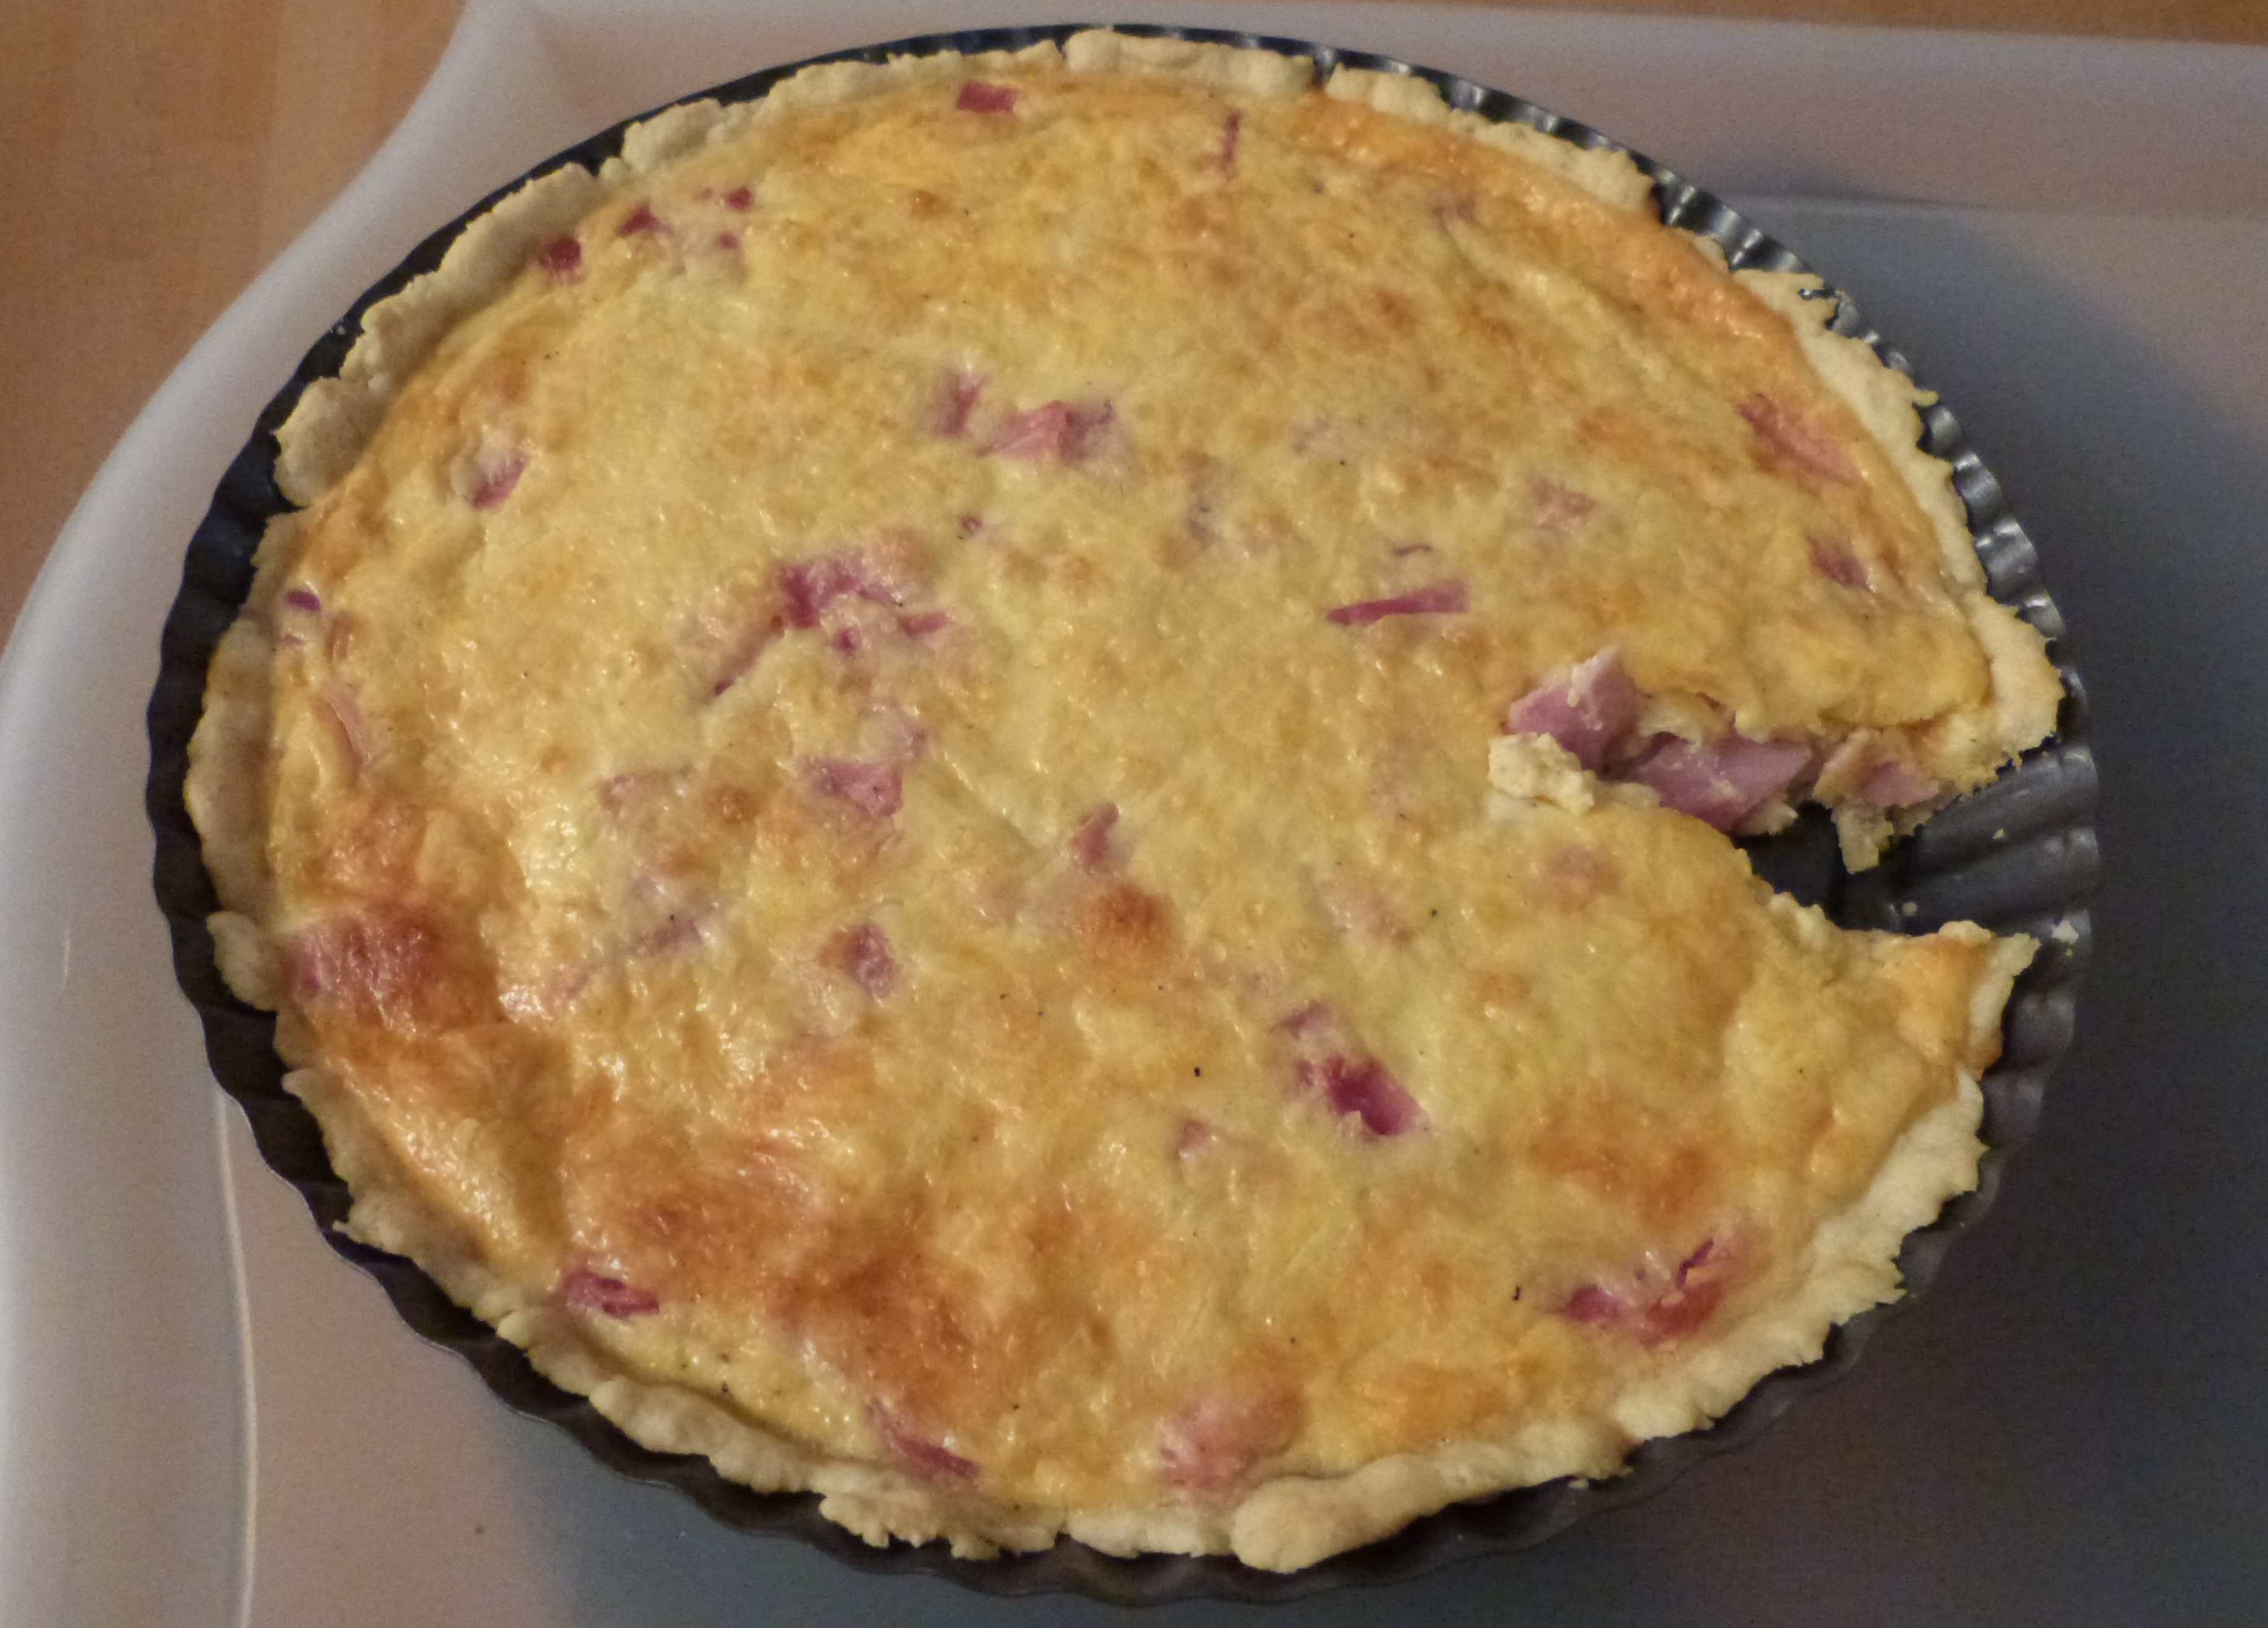
\includegraphics[width=\paperwidth,height=\paperheight]{./bilder/quiche_lorraine_ratio.jpg}};

\begin{recipe}[]{Quiche lorraine} % Mutti Feb 14 
	\timerecipe[Minuten]{ca. (60)+15+30} %mit [EINHEIT]
	\personcount[Personen]{2} % mit[ART]
	\ingredient{200g Mehl} % ggf. \nicefrac{1}{2}
	\ingredient{100g Butter}
	\ingredient{200g gekochter Schinken}
	\ingredient{3 Eier}
	\ingredient{\nicefrac{1}{4} Liter Sahne}
	\ingredient{125g geriebener Emmentaler}


\step
\textbf{200g Mehl}, \textbf{100g Butter}, \textbf{\nicefrac{1}{2} TL Salz} und \textbf{5 EL Wasser} zu einem Teig kneten und 1 Stunde kalt stellen.

\step
Backofen auf 200 Grad vorheizen.

\step
Teig in einer Springform ausrollen und mehrmals mit einer Gabel einstechen.

\step
\textbf{200g Schinken} in Streifen schneiden und auf dem Teig verteilen.

\step
\textbf{3 Eier}, \textbf{\nicefrac{1}{4} Liter Sahne} und \textbf{Pfeffer} verquirlen, die \textbf{125g geriebener Emmentaler} untermischen und auf dem Teig verteilen.

\step
Quiche auf der zweiten Schiene von unten ca. \nicefrac{1}{2} Stunde backen, bis sie eine schöne Farbe hat.


\tippbox{{Tipp:} Statt Schinken kann man auch gewürfelte Zuccinis oder Blattspinat oder in Scheiben geschnittene Champignons nehmen.} % Tipp in extra Rahmen
\end{recipe}